\chapter{The MAC layer}

\section{Introduction}

The MAC layer handles access to the same medium, avoiding collisions that cause
waste of time.
It has the following goals:
\begin{itemize}
\item efficiency in bandwidth use
\item avoid collisions (resilience)
\item fairness
\item robustness: the protocol should be decentralized
\item protocols easy to implement
\end{itemize}

\paragraph*{Typologies} The MAC layer has different typologies. As a matter of
fact, it offers different ways to share the channel: \textbf{TDMA}
(\textit{time division}), \textbf{FDMA} (\textit{frequency division}),
\textbf{CDMA} (\textit{code division}).
\paragraph*{Random access} MAC provides two way to randomly access the channel,
with \textbf{CSMA} (\textit{carrier sense multiple access}) and \textbf{MACA}
(\textit{multiple access with collision avoidance}).
\paragraph*{Other protocols} There are also ``taking turns'' MAC protocols, that
basically carries out a
polling scheme.

\subsection{Wired vs Shared Channel}

When the channel is a cable it's easier, because you just have to listen to it
before transmitting any data (this technique is called CSMA, \textit{Carrier
  sense  multiple access}\footnote{As an additional note, with CSMA you can
  even listen  when a collision happens.}): for example with Ethernet you can
check what you've sent and check if a collision happened. In a wireless
environment this is not possible, because when you're transmitting you can't
receive, otherwise you'll end up having a collision, but you can check if a
package has arrived to the destination with the ACKs\footnote{
  In wireless communications TCP packets are split into smaller packages of 100
  bytes each one when they arrive to the MAC layer: the ACKs are generated
  during transmission for the MAC layer and when a complete TCP packet is sent
  the receiver will generate a TCP response. Any TCP packet can generate one o
  more MAC packet, allowing the MAC layer to hide some losses to the top
  protocol. N.B.: this is not true for ad-hoc communications though.
}.

\section{MAC Layer approaches}

There are different ways the MAC layer can approach the access to the medium,
and these are:
\begin{itemize}
\item Random
  \begin{itemize}
  \item without carrier sensing (such as Aloha, Slotted Aloha)
  \item with carrier sensing (CSMA, CSMA/CD, MACAW)
  \end{itemize}
\item Controlled
  \begin{itemize}
  \item centralized (FDMA, TDMA, CDMA)
  \item distributed
  \end{itemize}
\end{itemize}

\subsection{Aloha}

This protocols was used to communicate between Hawaii islands. It doesn't have
synchronization, and the total throughput of this protocols is $\frac{1}{2e}$

\subsubsection{Slotted Aloha}

This version of Aloha has time divided slots: every transmission has to stay in
a defined time slot, that is not easy to do but it's possible. In case of a
collision, a re-transmission occurs with a probability $P$.

\paragraph*{Throughput} The throughput of this Aloha version with
synchronization is $\frac{1}{e}$

\subsubsection{Considerations about Aloha protocols}

In general, Aloha protocols have these common characteristics:
\begin{itemize}
\item not efficient
\item unfair
\item robust \& easy to implement
\end{itemize}

\subsection{CSMA}

With this approach, you first listen to the channel and then the protocol
algorithm tries to avoid transmission at the same time. CSMA comes with
different versions, based on the probability $p$ of transmission after the
channel becomes free.

\paragraph*{1-persistent CSMA} When the channel is free $\to$ transmit,
otherwise, wait until the channel becomes free. At this point, immediately
transmit. If a collision occurs, wait a random amount of time before
re-transmission.

It's easy to see that if two nodes are waiting the channel to become free they
will probably cause a collision because they will start transmitting at the
same time.

\paragraph*{non-persistent CSMA} Similar to 1-persistent CSMA, but if the
channel is busy then wait a random amount of time before checking it again.

\paragraph*{p-persistent CSMA} This version is slot based. If the channel is
free then the node transmits with a probability $p$, otherwise it waits a random
amount of time.

\subsubsection{CSMA/CD}

The CD version has a collision detection system, that allows to abort the
transmission when a collision is detected, reducing time wastage. This,
unfortunately, is \underline{not possible in wireless communications}, but only
in the wired one.

\paragraph*{SINR} SINR (\textit{signal-to-interference-plus-noise ratio})
is commonly used in wireless communication as a way to measure the quality of
wireless connections. Typically, the energy of a signal fades with distance,
which is referred to as a path loss in wireless networks.
Conversely, in wired networks the existence of a wired path between the sender
or transmitter and the receiver determines the correct reception of data. In a
wireless network ones has to take other factors into account (e.g. the
background noise, interfering strength of other simultaneous transmission). The
concept of SINR attempts to create a representation of this aspect\footnote{
\url{https://en.wikipedia.org/wiki/Signal-to-interference-plus-noise_ratio}
}.

The collision detection is based on the SINR and the formula to calculate it is:
\begin{equation}
SINR = \frac{Signal\ of\ Interest\ (SoI)}{Interference(I) + Noise(N)}
\end{equation}

The formula to calculate the SINR between two nodes (given interference between
C and B) is:
\begin{equation}
SINR^{A}_{B} = \frac{\frac{P^{A}_{transmit}}{d^{\alpha}_{AB}}}{N + \frac{P^{C}_{transmit}}{d^{\alpha}_{CB}}}
\end{equation}

\begin{figure}[t]
  \centering
  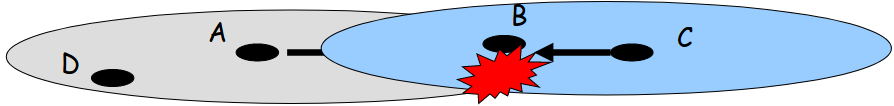
\includegraphics[scale=0.4]{SINR1}
  \caption{An example of a collision detection}
\end{figure}

In this formula $P^{X}_{transmit}$ represents the power transmission of X, and
$d^{\alpha}_{XY}$ is the \textit{SoI} between $X$ and $Y$. The noise ($N$) is
somehow a fixed value.

The nodes position and the signal interference cause communication problems in
wireless networks, e.g. the \textbf{hidden terminal problem} and the \textbf{
  exposed terminal problem}, that will be explained in the next part.

\section{Communication problems with wireless networks}

As already mentioned, there are problems with wireless networks related to the
nodes' position and the strength of the signal that will be explained here.

\subsection{Hidden terminal problem}

The hidden node problem occurs when a node is visible from a wireless access
point (AP) but not from other nodes communicating with that AP, due to
difficulties in the media access control sub-layer.

\begin{figure}[t]
  \centering
  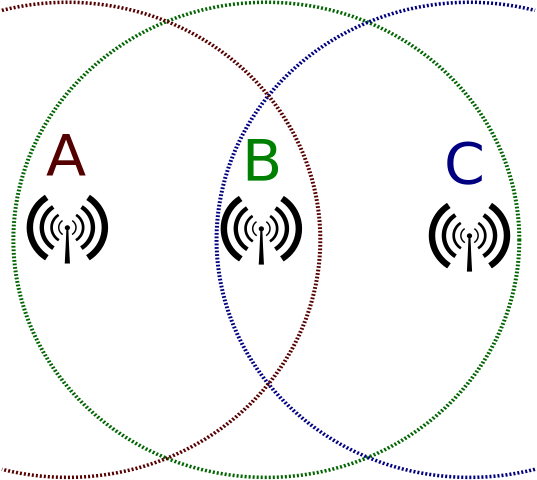
\includegraphics[scale=0.25]{WifiHiddenStationProblem}
  \caption[Hidden terminal problem]{Hidden terminal problem. Station A can
    communicate with Station B. Station C can also communicate with Station B.
    However, Stations A and C cannot communicate with each other since they
    cannot sense each other on the network, because they are out of range of
    each other.}
\end{figure}

\subsection{Exposed terminal problem}

Exposed node problem occurs when a node is prevented from sending packets to
other nodes because of a neighboring transmitter.

\begin{figure}[t]
  \centering
  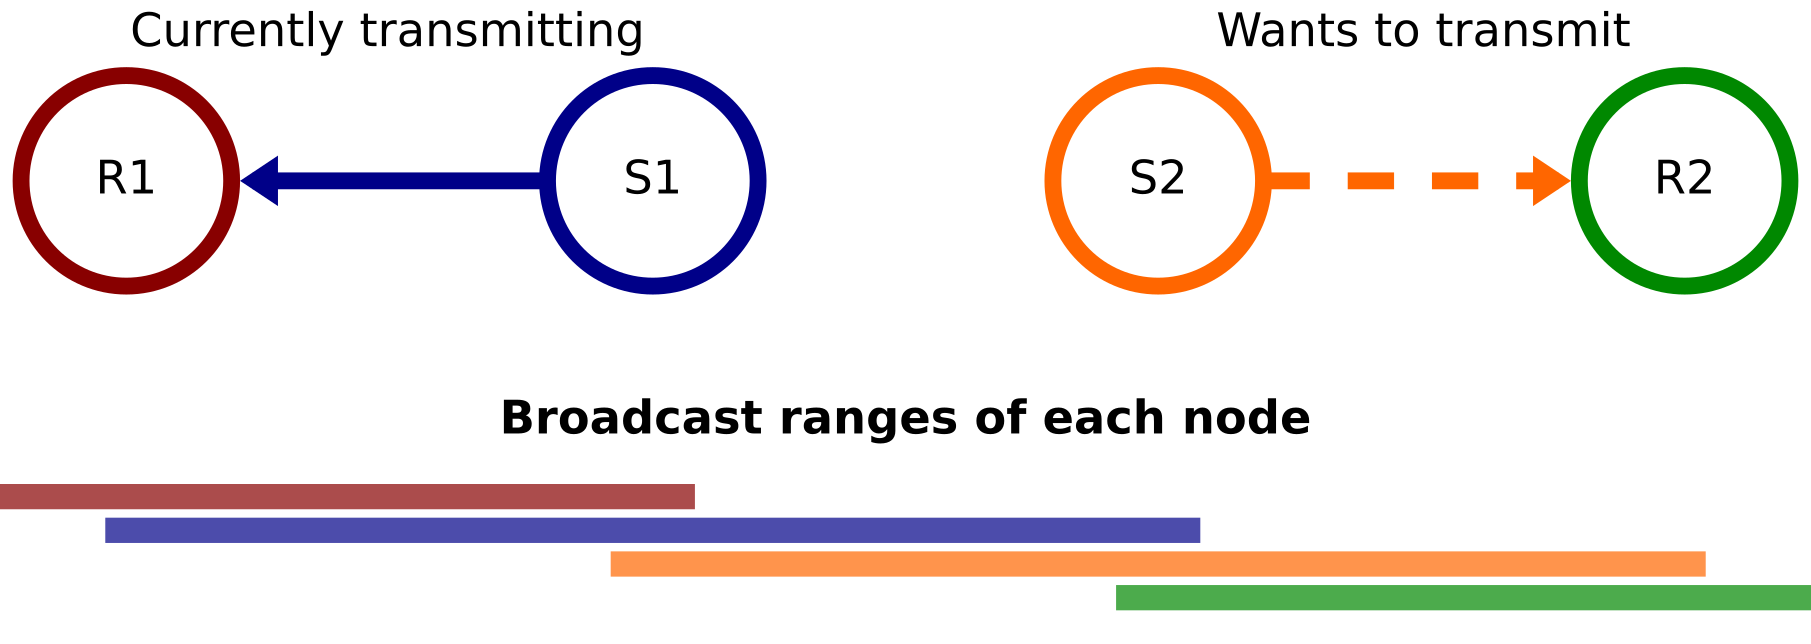
\includegraphics[scale=0.8]{WifiExposedStationProblem}
  \caption[Exposed terminal problem]{Exposed terminal problem. Station S2
    wants to communicate with R2, but has sensed S1 that's currently
    transmitting to R1 so it doesn't transmit for not causing a collision. In
    this case, though, S2 should not defer transmission to R2 because this won't
    create any interference with S1's transmission.}
\end{figure}

\subsection{MACAW} \todo{This part is very confused, since the slides are a
  cluster-fuck of information randomly thrown. Please check out \underline{very
    closely} and critically this content because I'm not sure of what I'm
  writing!}

Given that wireless MAC proved to be non-trivial, in 1994 a research lead by
Bhargavan made MACAW (\textit{Multiple Access with Collision Avoidance for
  Wireless}) that now is used for congestion avoidance. It has the same
operating principle of 802.11, and it's widely used in ad-hoc networks.
MACAW helps solving the hidden terminal problem, but not the exposed terminal
problem.

\paragraph*{Channel access method}
MACAW uses CTS and RTS packets to knowing if the channel is free to be used to
transmit new data. These two types of packets are very small, so it's difficult
to have a collision transmitting them.

\subparagraph*{RTS} \textit{Request to Send} is a frame sent by the
sender to the receiver before starting a transmission that asks if there are no
current transmission that could interfere with the new one

\subparagraph*{CTS} \textit{Clear To Send} is a frame sent by the receiver
that informs the sender that there is a possibility to use the channel to start
a new transmission.

\begin{figure}[t]
  \centering
  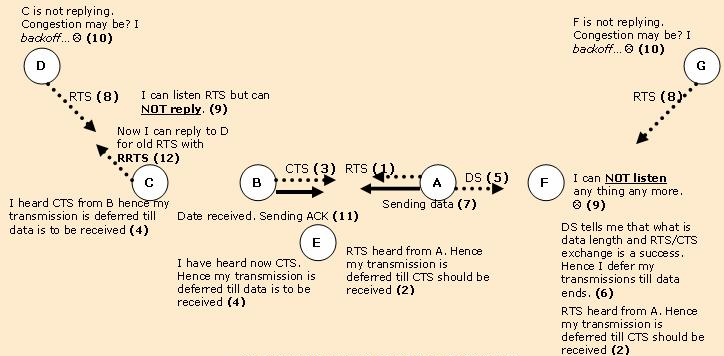
\includegraphics[scale=0.75]{MACAW}
  \caption{A schema describing an example of how MACAW works}
  \label{fig:mac:macaw}
\end{figure}

\subparagraph*{How it works} From Figure~\ref{fig:mac:macaw}, assume that node A
has data to transfer to node B.
Node A initiates the process by sending a Request to Send frame (RTS) to node B.
The destination node (node B) replies with a Clear To Send frame (CTS). After
receiving CTS, node A sends data. After successful reception, node B replies
with an acknowledgment frame (ACK). If node A has to send more than one data
fragment, it has to wait a random time after each successful data transfer and
compete with adjacent nodes for the medium using the RTS/CTS mechanism.

Any node overhearing an RTS frame (for example node F or node E in the
illustration) refrains from sending anything until a CTS is received, or after
waiting a certain time. If the captured RTS is not followed by a CTS, the
maximum waiting time is the RTS propagation time and the destination node
turnaround time.

Any node (node C and node E) overhearing a CTS frame refrains from sending
anything for the time until the data frame and ACK should have been received
(solving the hidden terminal problem), plus a random time. Both the RTS and CTS
frames contain information about the length of the DATA frame. Hence a node uses
 that information to estimate the time for the data transmission completion.

Before sending a long DATA frame, node A sends a short Data-Sending frame (DS),
which provides information about the length of the DATA frame. Every station
that overhears this frame knows that the RTS/CTS exchange was successful. An
overhearing station (node F), which might have received RTS and DS but not CTS,
defers its transmissions until after the ACK frame should have been received
plus a random time.

To sum up, a successful data transfer (A to B) consists of the following
sequence of frames:
\begin{enumerate}
\item ``Request To Send'' frame (RTS) from A to B
\item ``Clear To Send'' frame (CTS) from B to A
\item ``Clear To Send'' frame (CTS) from B to A
\item ``Data Sending'' frame (DS) from A to B
\item DATA fragment frame from A to B, and
\item Acknowledgment frame (ACK) from B to A.\footnote{
Taken from
\url{https://en.wikipedia.org/wiki/Multiple_Access_with_Collision_Avoidance_for_Wireless}
}
\end{enumerate}

\subparagraph*{MILD Algorithm} MACAW uses contention windows (\textit{cw}) to
determine the packet transmission rate. When a node fails to receive CTS in
response to its RTS it multiplies his contention window by $1.5$. This approach
is less aggressive than 802.11, which multiplies by $2$. When a node
successfully completes a transfer, it reduces the contention window by
$1$\footnote{That reduction could be a little too conservative.}. This avoids
wild oscillation of the contention window when congestion is high.
The congestion window helps with the fairness: when a node transmits the
packet it appends its current congestion windows, that is used by the others
for future transmission output.

\paragraph*{Fairness}
There are two main ways to establish fairness in MACAW, via \textit{Weighted
  fair queuing} and via \textit{Distributed fair scheduling (DFS)}.

\subparagraph*{Weighted fair queuing} Each node has a weight in order to have a
bandwidth usage proportional to it

\subparagraph*{DFS} The \textit{Distributed fair scheduling}:
\begin{itemize}
\item chooses back-off intervals proportional to packet size/weight
\item works well on LAN
\item always include some randomness
\end{itemize}

\paragraph*{Scanning} Scanning it obviously join, find and initialize a network.
It can be of 2 typologies:
\begin{itemize}
\item active: the client actively search for beacons
\item passive: the AP sends beacons continuously
\end{itemize}

\section{MAC for 802.11}
\paragraph*{802.11} The 802.11 protocol is used mostly indoor, it uses three
bands (900 MHz, 2.4GHz, 5GHz) and its applications are related to nomadic
internet access, portable computing and ad-hoc networking.
802.11 has two types of configurations:
\begin{itemize}
\item with a base station (control station, access point)
\item ad-hoc networking (point-to-point)
\end{itemize}

\paragraph*{Steps for establishing a connection}
The steps for establishing a connection through the MAC protocol in 802.11 are:
\begin{enumerate}
\item[1] DIFS (\textit{Distributed Inter Frame Space}): time where the channel
  has to be free. If a node gains access to the channel goes to step 2a,
  otherwise to step 2b.
\item[2a] Data transmission
\item[2b] NAV (\textit{Network Allocation Vector}): time where the others have
  to wait before starting another transmission
\item[3] SIFS (\textit{Short Inter Frame Space}): time where the channel has to
  be free
\item[4] MAC ACK
\end{enumerate}

\subsection{Channel connection \& priorities}
Channel contentions can be of the following typologies:
\begin{itemize}
\item SIFS
\item PIFS (only with polling schema)
\item DIFS
\end{itemize}

The contention time starts before the next frame and after SIFS/PIFS/DIFS
occurs.
The packages transmission order is the following:
\begin{AutoMultiColEnumerate}
\item DIFS
\item RTS
\item SIFS
\item CTS
\item SIFS
\item Data
\item SIFS
\item ACK
\end{AutoMultiColEnumerate}

\subsection{Access methods}
802.11 has different access methods:
\begin{itemize}
\item MAC-DCF CSMA/CA (mandatory)
\item MAC-DCF with RTS/CTS (optional)
\item MAC-PCF (polling the AP) (optional)
\end{itemize}

\paragraph*{CSMA} CSMA doesn't entirely solve the hidden/exposed terminal
problem. The CSMA doesn't work well with the hidden terminal, so a CA
(collision avoidance) solution is used. This adds two packets before data
transmission, RTS and CTS. These packets are very little, thus fast to transmit.

\subparagraph*{Congestion avoidance} The congestion avoidance works in this way:
\begin{itemize}
\item DCF: distributed control function
\item Countdown of random back off suspended if the medium is busy (it's not
  reset!)
\item The CW (contention window) is \underline{larger}\footnote{Large $cw$ cause
  large overhead} when there are many nodes, \underline{smaller} if fewer. When
  a node fails to receive CTS in response to its RTS, it doubles the
  contention windows.
\end{itemize}

\paragraph*{PCF} With this access method the AP announces it in the beacons.
After associations frames the node announces to the AP whether it's pollable
and capable to transmit during the contention free period (CFP).

\subparagraph*{Power Management}
Stations are allowed to go to sleep and this state is saved in the AP memory.
Pay attentions to the fact the the energy a node consumes to wake up is more
that the one it uses to stay asleep, if it wakes up too often. Sleep is intended
for long times.

When a node sleeps, the packets for it are buffered in the AP. When it wakes up,
it downloads all the packages not yet received. TSF (\textit{time
  synchronization function)} assures AP and power save stations are
synchronized.
